\section{Scrum}
Scrum is a framework for teams of developers who are involved in the development of complex projects.
Teams should be self-organizing with associated roles. A team has the skills to accomplish the work and
Scrum is designed to optimize flexibility and productivity. This methodology is rapidly becoming the standard
in companies who develop software and makes sense for students who are about to go into the real world of
software development to learn it. Also, this project generally specifies Scrum as the project methodology to be used.

\subsection{Roles}

Scrum distinguishes between the Scrum master, the product owner and the development team.

Scrum Master position means an individual who will be responsible for the product in a
particular sprint, as well as liaise between the team and the product owner.
A Scrum Master is responsible for making sure that the team adhere to the Scrum guidelines,
and should never be seen as the boss of the group, but instead as the coach.
She should also make sure that the team is on the right track keeping a constant eye on the sprint goal
and the definition of "done" for the different tasks.

Product Owner position means an individual who is considered to be the client in the project.
The Product Owner is the person who owns and controls the development of the software with the help of the backlog,
prioritizing features and generally the one who is supposed to give you the direction in sprint planning and demos.

The Development Team is the set of individuals who are working on the code for the product owner.
The team is responsible for creating increments and releasing a working version of the software
in each sprint.

\subsection{Scrum Keywords}
\begin{itemize}
\item{\textbf{User story}}\\
A user story is defined as a function the system must provide to the end user.
A user requirement is translated to a user story so that the developer does know exactly
what the user needs to accomplish for that function and why she needs it. User stories are usually
broken down to tasks and each task is the smallest work unit to implement.
It is important that the developer team agrees on the definition of "done" for each story.

\item{\textbf{Product backlog}}\\
The product backlog is an ordered list of user stories. Stories are usually prioritized by the product owner 
depending on criteria such as date needed or business value.

\item{\textbf{Standup meetings}}\\
A mandatory short meeting (usually 10 minutes) starting every day at the same time.
Each person tells the others what she did the day before and what she is going to do
next. The participants attend the meeting standing so that everyone is encourage to be concise
when telling the status of their work. Standup meetings are a great way to ensure continuous
synchronization among the members of a team.

\item{\textbf{Sprint}}\\
A sprint is the core artifact of Scrum. A sprint is an iteration that usually lasts between one or two weeks
during which a part of an entire product is implemented. Each sprint has a goal and each member of
the team should strive to fullfill that goal. The whole project period consists of several sprints.

\item{\textbf{Sprint backlog}}\\
A list of stories that should be completed during a sprint. The sprint backlog is filled by picking stories
from the product backlog.

\item{\textbf{Sprint planning}}\\
In the beginning of each sprint the team meets for planning and to agree on the goal to achieve in the iteration.
Stories are picked from the product backlog and broken down to tasks, and the team makes an estimation of the workload
for each task so that the work can be completed during the time allocated for the sprint.

\item{\textbf{Srint demo}}\\
Present the result of the sprint in the form of a working product to the customer.

\item{\textbf{Sprint retrospective}}\\
After each sprint is completed, the team gather to discuss the completed sprint, trying to reflect on the good and bad parts
of the sprint. The output of the meeting is used for improving the project flow and the work within the group.
\end{itemize}

\pagebreak

\subsection{Scrum process}
The following picture summarize the Scrum methodology.

\begin{figure}[!h]
\centering
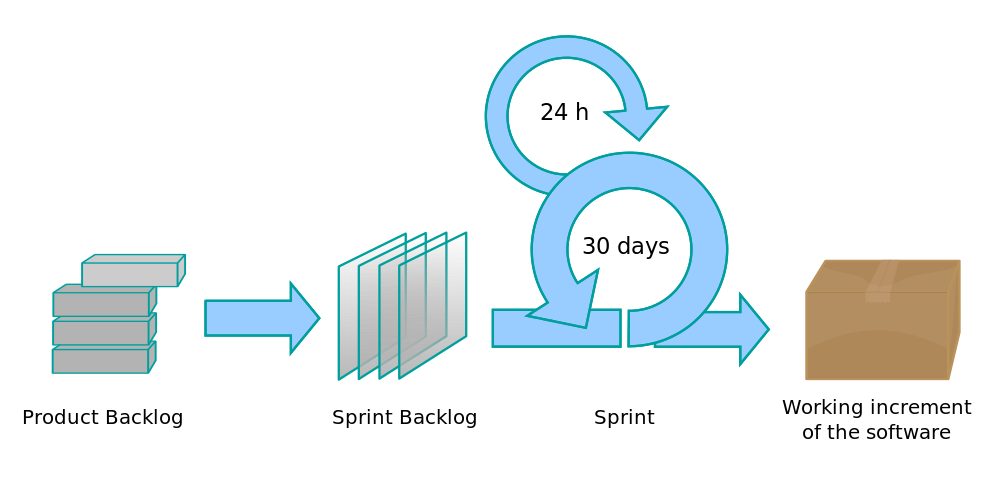
\includegraphics[scale=0.35]{graphics/scrum.png}
\caption{The Scrum Process}\label{fig:scrum_process}
\end{figure}
